

In this section we demonstrate that the proof system presented in section \ref{sect:proofSystem} is sound. 
For this, we give a stronger, deeper meaning to our Hoare tuples  (Sect \ref{s:deep:valid}), which requires that satisfaction of assertions is preserved from the perspective of several frames, rather than just the top frame.

We prove soundness of of Hoare triples (Sect \ref{sect:prove:triples:sound}).
We then show how execution starting from some external state can be summarised into purely external execution and terminating execution of public methods (Sect \ref{sect:termExecs}). We then use these decompositions and a well-founded ordering to prove soundness of our quadruples  and of the overall system (Sect \ref{sect:prove:sound:quadruples}).


\subsection{Deep Satisfaction} 
\label{s:deep:valid}


Per section~\ref{s:viewAndProtect}, an assertion may hold in one state
but not afterwards.

\begin{example}
\label{ex:motivate:deep}
Assume state $\sigma_a$, such that $\interpret {\sigma_a} {\prg{this}}=o_1$, $\interpret {\sigma} {\prg{this}.f}=o_2$, $\interpret {\sigma} {x}=o_3$, $\interpret {\sigma} {x.f}=o_2$,  
and $\interpret {\sigma} {x.g}=o_4$, where $o_2$ is external and all other objects are internal. 
We then have $..,\sigma_a \models  \inside {o_4}$.
Assume that the continuation of $\sigma_a$   consists of a method $x.m()$. Then,
upon entry to that method, when we push the new frame, we have a state $\sigma_b$, which also satisfies $..,\sigma_a \models  \inside {o_4}$.
Assume that the   body of $m$ is $\prg{this}.f.m1(\prg{this}.g); \prg{this}.f := \prg{this};  \prg{this}.g := \prg{this}$, and that the external method $m1$ stores in the 
receiver a reference to the argument.
Then, at the end of method execution, and before popping the stack, we have a state $\sigma_c$, which also satisfies $..,\sigma_c \models  \inside {o_4}$.
However, after we pop the stack, we obtain $\sigma_d$, for which $..,\sigma_d \not\models  \inside {o_4}$.
\end{example}
 

To address this problem, we introduce ``deep satisfaction'' of assertions $ \satDAssertFrom M  \sigma k   A$ which says that $A$ is satisfied in $\sigma$  in all frames of $\sigma$ from $k$ onwards, 
\ie  $ \satDAssertFrom M  \sigma k   A$ iff $\sigma = ((\phi_1\cdot ... \phi_n), \chi)$ and $k\leq n$ and $\forall j. [\  k\leq j \leq n \ \Rightarrow \ M, ((\phi_1\cdot ... \phi_j), \chi) \models A'\ ]$ where $A'$ is $A$ where all free variables have been substituted according to $\phi_n$ -- \cf Def. \ref{def:restrict}.
We then introduce ``deep'' quadruples,   $\satisfiesD {M} {\quadruple  {A} }   {\sigma}   {A'} {A''}$ , which promise that if $\sigma$ satisfies $A$ from $k$ onwards, and executes its continuation to termination, then the final state will satisfy $A'$ from $k$ onwards, and also, all intermediate external states will satisfy $A''$ from $k$ onwards - \cf Def \ref{def:restrict}.
We define   $\satisfiesD {M} {\quadruple  {A} }   {stmt}   {A'} {A''} $ and  $\satisfiesD {M} {S}$ accordingly.


Thus. continuing with example \ref{ex:motivate:deep},  we have that\ \  $\satisfies {M} {\quadruple   {\inside {o_4}} }   {\sigma_b}   {\inside {o_4}}  {true} $, \ \ 
 but \\ $\notSatisfiesD {M}   {\quadruple   {\inside {o_4}} }  {\sigma_b}   {\inside {o_4}}  {true}  $.
\ \  In general, deep satisfaction is stronger than shallow:   
 
\begin{lemma}[Deep   vs Shallow Satisfaction]
For all $M$, $A$, $A'$, $A''$, $\sigma$, $stmt$, and $S$
\begin{itemize}
\item
 $\satisfiesD {M} {\quadruple  {A} }   {\sigma}   {A'} {A''}   \ \ \ \Longrightarrow \ \ \   \satisfies {M} {\quadruple  {A} }   {\sigma}   {A'} {A''}$

\item
 $\satisfiesD {M} {\quadruple  {A} }   {stmt}   {A'} {A''}   \ \ \ \Longrightarrow \ \ \   \satisfies {M} {\quadruple  {A} }   {stmt}   {A'} {A''}$
\item 
$\satisfiesD {M} {S}  \ \ \ \Longrightarrow \ \ \ \satisfies {M} {S}$
\end{itemize}
\end{lemma}


%%%%%%%%%%%%%%%%%%%%%%%%%%%%%%%%%%%%%%%%%%%%%%%%%%%

 \subsection{Expectations}

We require a  proof system for assertions, $M\vdash A$, and expect it to be sound.
We also require
an   underlying Hoare logic, $M\ \vdash_{ul}\  \triple A {stmt} {A'}$, and expect it to be be  sound:
\begin{axiom}
\label{lemma:axiom:enc:assert:ul}
\label{ax:ul:sound}
We require a sound logic of assertions ($M \vdash A$), and a sound Hoare logic , \ie that for all $M$, $A$, $A'$, $stmt$:
\begin{center}
$M \vdash A   \ \ \ \  \Longrightarrow  \ \ \ \  \forall \sigma.[\ M, \sigma \models A\ ]$.\\
% \end{center}
%\end{axiom}
%
%\noindent
%Moreover, we assume that the  \ie for all $A$, $A'$, $stmt$:\ \ \  
%
%\begin{axiom}
% \begin{center}
{$M\ \vdash_{ul}\  \triple A {stmt} {A'}  \ \ \ \  \Longrightarrow  \ \ \ \ \satisfies  {M} { \triple A {stmt} {A'}}$ }
 \end{center}
\end{axiom}


%%%%%%%%%%%%%%%%%%%%%%%%%%%%%%%%%%%%%%%%%%%%%%%%%%%

\subsection{Soundness of the Hoare Triples Logic}

\label{sect:prove:triples:sound}
We prove various properties about protection
\cf section \ref{s:app:protect:lemmas}.
Using these lemmas. we prove soundness of the inference system for triples $M \vdash  \triple A {stmt} {A'} $ -- \cf \A, \ref{s:sound:app:triples}.

 

\begin{Theorem}
\label{l:triples:sound}
For module  $M$ % and $\Mtwo$, 
such that  $\vdash M$, and for any assertions $A$,  $A'$, $A''$ and statement  $stmt$:
\begin{center}
$M\ \vdash\  \triple A {stmt} {A'}  \ \ \ \  \Longrightarrow  \ \ \ \ \satisfiesD {M} {\quadruple {A} {stmt} {A'} {A''}}$
\end{center}
\end{Theorem}
 

\subsection{Summarised Execution}

When proving soundness of the external call rule, we are faced with the following challenge; 
%For the soundness proof of our quadruples we need to address two challenges:
Execution of an external call may consist of any number of external
steps, interleaved with calls to public internal methods, which in
turn may may make any number of further internal call (whether public or private), and these, again may call external methods.
 

, etc\ldots% leading to further calls of public methods.
%
We address the second challenge by introducing summarised executions, which essentially collapse all public, internal method calls into one large step (\cf Section \ref{sect:termExecs}).

\subsubsection{A well-founded ordering}
\label{sect:prove:wellfounded}

We define that $(A_1,\sigma_1,A_2, A_3) \ll_{M,\Mtwo}  (A_4,\sigma_2,A_5, A_6)$ if $\sigma_1$ executes to terminations in fewer steps than $\sigma_2$ considering the shortest, terminating scoped execution), or  the proof of $M \vdash \quadruple {A_1} {\sigma.\prg{cont}} {A_2} {A_3} $
is shallower than the the proof of  $M \vdash \quadruple {A_4} {\sigma.\prg{cont}} {A_5} {A_6} $ (considering the shallowest possible proofs). Full Def. in \ref{def:measure}.

 

 


\begin{auxLemma}
\label{lemma:normal:two}
For any modules $M$ and $\Mtwo$,  the relation $\_ \ll_{M,\Mtwo}  \_$ is well-founded.
\end{auxLemma}

%%%%%%%%%%%%%%%%%%%%%%% S U M M A R I E S of exectuon %%%%%%%%%%%%%%%%%%%%%%%%%%%%%%%%%%%%%%%%%%%%% 
\subsubsection{Summarised  execution} 
\label{sect:termExecs}

In this subsection we prove auxiliary lemmas that allow us to summarise execution into  constituent parts, which are useful for the proof of soundness of our quadruples, Theorem \ref{t:quadruple:sound}, when we consider sequences of statements, and also method calls.

%We prove some unsurprising 
% DO we need it?
%Lemma \ref{lemma:encl:tem} guarantees that any state reachable from a state with a terminating execution has itself a terminating execution, and that this execution is enclosed in the original one:
% Lemma \ref{lemma:subexp} makes the usual guarantee about terminating execution of statement sequences.
 


\label{sect:termExecs}

The challenge in the proof of soundness of our quadruples, Theorem \ref{t:quadruple:sound} is the proof of external calls. 
Namely, an external call may eventually call any number of public, internal, methods, which , in turn, may make further external calls.
Thus, an external call will involve several internal and external states.

\vspace{.1cm}

\begin{tabular}{lll}
\begin{minipage}{.45\textwidth}
The diagram to the left shows such an execution, where
  $ \leadstoBoundedStarFin {\Mtwo\cdot M}    {\sigma_2}  {\sigma_{30}}$ consists of 4 calls to external objects,
and 3 calls to internal objects.
The calls to external objects are from $\sigma_2$ to $\sigma_3$,  from $\sigma_3$ to $\sigma_4$, from $\sigma_9$ to $\sigma_{10}$, 
and  from $\sigma_{16}$ to $\sigma_{17}$.
 The calls to internal objects are from $\sigma_5$ to $\sigma_6$, rom $\sigma_7$ to $\sigma_8$, and from $\sigma_{21}$ to $\sigma_{23}$. 
\end{minipage}
& \ \  &
\begin{minipage}{.4\textwidth}
\resizebox{6.2cm}{!}
{
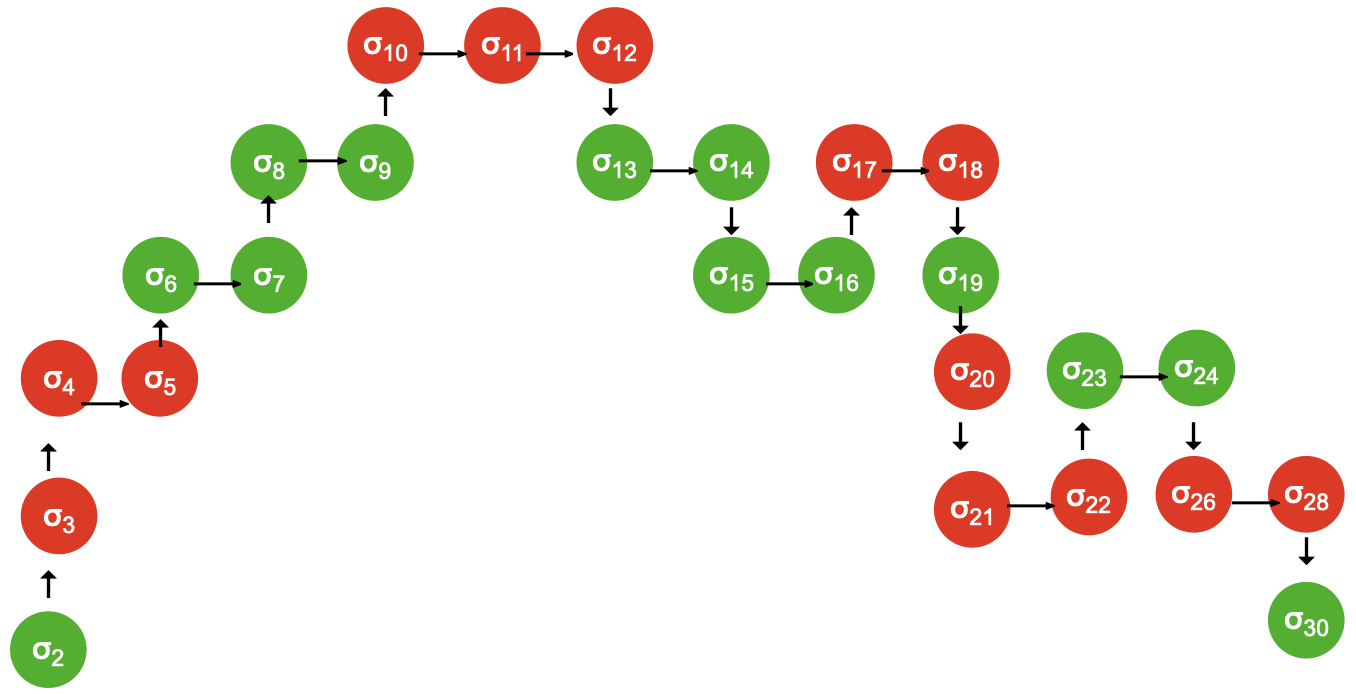
\includegraphics[width=\linewidth]{diagrams/summaryA.png}
} \end{minipage}
\end{tabular}
 
\vspace{.1cm}

When proving soundness of the rule {\sc{Call\_Ext}}, % and  {\sc{Call\_Ext\_Adapt}}
we will use that  $M \vdash \encaps A$ (and also deep satisfaction)  to argue that 
external transitions (from one external call to another) will preserve $A$. 
For the internal calls, we want to just apply the fact that the method body has been proven to preserve $A$ (by  {\sc{MEthod}}).
That is, for the external states we consider small steps, while for each of the public method calls we consider large steps. 
Moreover, for the external states we apply different arguments than for the internal states.

\vspace{.1cm}

\begin{tabular}{lll}
\begin{minipage}{.45\textwidth}
 In terms of our example, we want to summarise the execution of the two ``outer'' internal, public methods into the 
 ``large'' steps $\sigma_6$ to $\sigma_{19}$ and $\sigma_{23}$ to $\sigma_{24}$.
 And are not concerned with the states reached from these two public method executions.  
\end{minipage}
& \ \  &
\begin{minipage}{.4\textwidth}
\resizebox{6.2cm}{!}
{
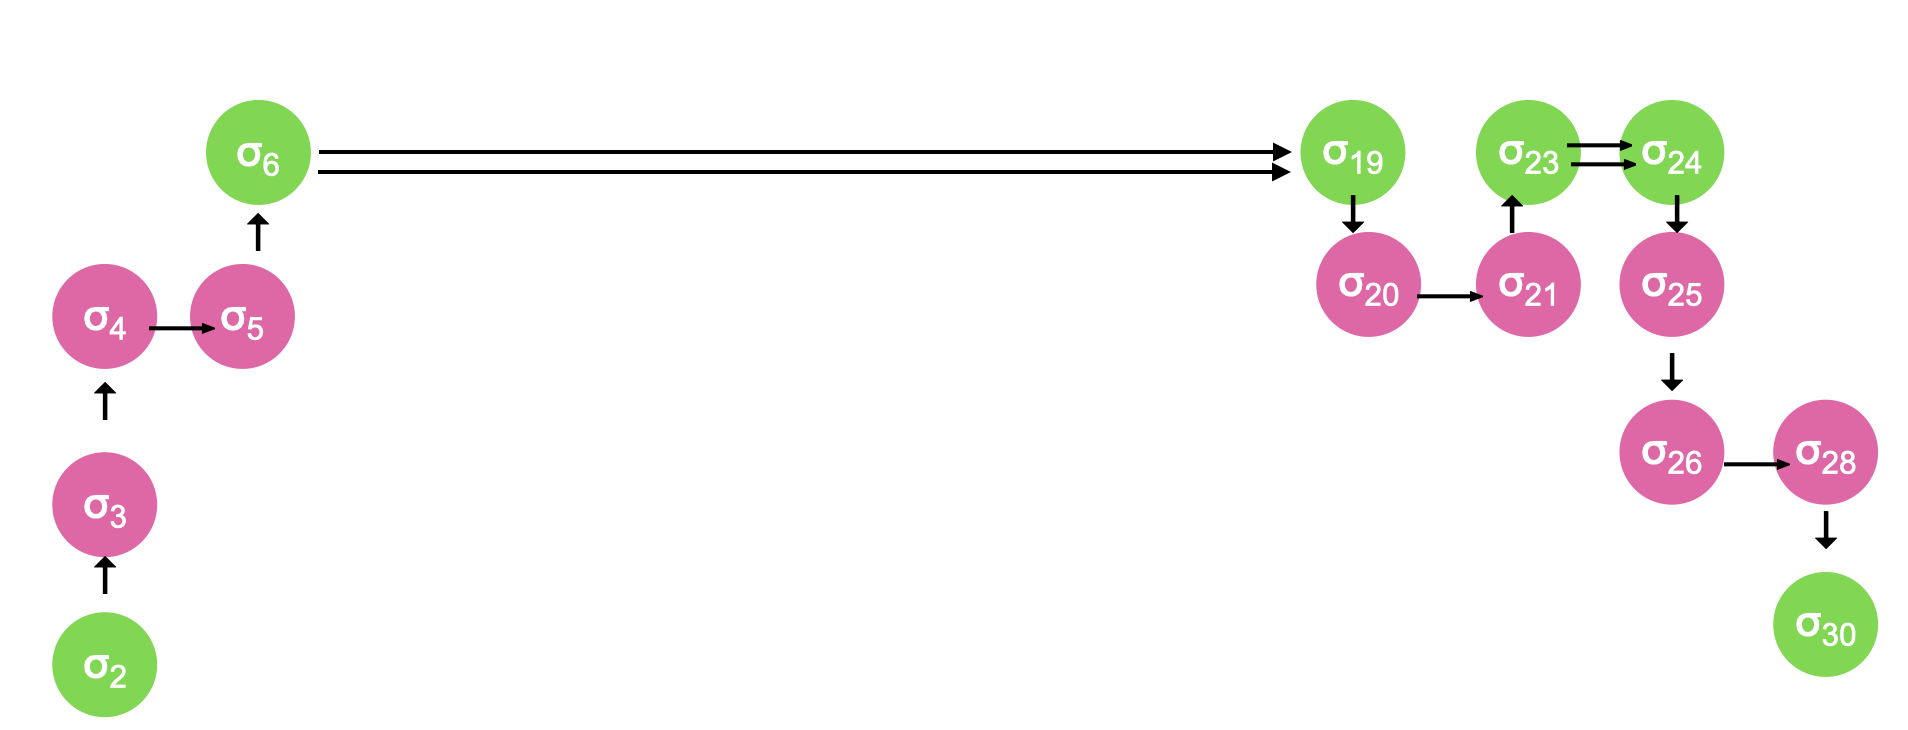
\includegraphics[width=\linewidth]{diagrams/summaryB.png}
} \end{minipage}
\end{tabular} 

 \vspace{.15cm}

\noindent 
In order to express such summaries, Def. \ref{def:exec:sum} introduces the following concepts:
\begin{itemize}
\item
 ${\leadstoBoundedThreeStarExt {\Mtwo\cdot M} {\sigma\bd}  {\sigma}  {\sigma'}}$ \ \ \  execution from $\sigma$ to $\sigma'$ scoped by $\sigma\bd$, involving  external states.
\item
${\WithPub {\Mtwo\cdot M}    {\sigma}  {\sigma'} {\sigma_1}}$ \  \ \  \ \ \ \ \ \ \ \  ${\sigma}$ is an external state  calling an internal public method, and \\
$\strut \hspace{3.25cm}$ $\sigma'$ is the state after return from the public method, and \\
$\strut \hspace{3.25cm}$  $\sigma_1$ is the first state upon entry to the public method.  
%$\WithExtPub {\Mtwo\cdot M} {\sigma\bd}  {\sigma}  {\sigma'} {\epsilon}$ \ \     \ \  $\triangleq$ \ \ 
%$\leadstoBoundedThreeStarExt {\Mtwo\cdot M} {\sigma\bd}  {\sigma}  {\sigma''}$
%\item
%$\WithExtPub {\Mtwo\cdot M} {\sigma\bd}  {\sigma}  {\sigma'} {\sigma_1...\sigma_n}$   \ \  int
%\item
%$\leadstoBoundedExtPub {\Mtwo\cdot M}    {\sigma}  {\sigma'} $   \ \ \ \ \   \ \ \  \ \ \ \   \ \ \ \  $\triangleq$   \ \ 
%  $ \exists n\in \mathbb{N}. \exists \sigma_1,...\sigma_n. \ \WithExtPub {\Mtwo\cdot M} {\sigma}  {\sigma}  {\sigma'} {\sigma_1...\sigma_n} 
%$
\end{itemize}
  
Continuing with our example, we have the following execution summaries:
\begin{enumerate}
\item
${\leadstoBoundedThreeStarExt {\Mtwo\cdot M} {\sigma_3}  {\sigma_3}  {\sigma_5}}$\ \ \ 
Purely external execution from $\sigma_3$ to $\sigma_5$, scoped by $\sigma_3$.
\item
${\WithPub {\Mtwo\cdot M}    {\sigma_5}  {\sigma_{20}} {\sigma_{6}}}$. \ \ \ 
Public method call from external state $\sigma_5$ into  nternal state $\sigma_6$ returning to $\sigma_{20}$. 
Note that this   summarises two  internal method executions ($\sigma_{6}-\sigma_{19}$, and $\sigma_8-\sigma_{14}$),
and two external method executions ($\sigma_{6}-\sigma_{19}$, and $\sigma_8-\sigma_{14}$).
\item
 ${\leadstoBoundedThreeStarExt {\Mtwo\cdot M} {\sigma_3}  {\sigma_{20}}  {\sigma_{21}}}$.
 \item
${\WithPub {\Mtwo\cdot M}    {\sigma_{21}}  {\sigma_{25}} {\sigma_{23}}}$. \ \ \ 
Public method call from  external state ${\sigma_{21}}$ into internal state $\sigma_{23}$, and returning to external state $\sigma_25$.
 \item
  ${\leadstoBoundedThreeStarExt {\Mtwo\cdot M} {\sigma_3}  {\sigma_{25}}  {\sigma_{28}}}$.
\ \ \ 
  Purely external execution from $\sigma_{25}$ to $\sigma_{28}$,, scoped by ${\sigma_3}$.
\end{enumerate}

\vspace{.1cm}
\noindent
Finally, Def. \ref{def:exec:sum} also defines:
\begin{itemize}
\item
$\WithExtPub {\Mtwo\cdot M} {\sigma\bd}  {\sigma}  {\sigma'} {\sigma_1...\sigma_n}$  \ \ purely external executions, interleaved with summarised public internal method calls, starting at ${\sigma_1...\sigma_n}$, respectively.
\end{itemize}

In terms of our example, we have that \ \ \ $\WithExtPub {\Mtwo\cdot M} {\sigma_2}  {\sigma_{2}}   {\sigma_{20}}  {\sigma_5,\sigma_{21}}$.


  


  %%%%%%%%%%%%%%%%%%%%%%%%%%%%%%%%%%%%%%%%%%%%%%%%%%%

\subsection{ Soundness of the Hoare Quadruples Logic}

Another challenge when proving soundness of our quadruples, is that in some cases we want to 
%For the soundness proof of our quadruples we need to address two challenges:
apply induction on the execution and  in other cases we want to apply induction on the Hoare logic
proof.  We address this challenge  through the definition of a well-founded ordering (\cf Section \ref{sect:prove:wellfounded}). 

\subsubsection{A well-founded ordering}
\label{sect:prove:wellfounded}

We define that $(A_1,\sigma_1,A_2, A_3) \ll_{M,\Mtwo}  (A_4,\sigma_2,A_5, A_6)$ if $\sigma_1$ executes to terminations in fewer steps than $\sigma_2$ considering the shortest, terminating scoped execution), or  the proof of $M \vdash \quadruple {A_1} {\sigma.\prg{cont}} {A_2} {A_3} $
is shallower than the the proof of  $M \vdash \quadruple {A_4} {\sigma.\prg{cont}} {A_5} {A_6} $ (considering the shallowest possible proofs). Full Def. in \ref{def:measure}.


\begin{auxLemma}
\label{lemma:normal:two}
For any modules $M$ and $\Mtwo$,  the relation $\_ \ll_{M,\Mtwo}  \_$ is well-founded.
\end{auxLemma}

\label{sect:prove:sound:quadruples}
We now prove soundness of the inference system $M \vdash  \quadruple A {stmt} {A'} {A''}$, using the decomposition of execution from the earlier section, and the ordering defined in Def. \ref{lemma:normal:two}.

\noindent
Lemma \ref{lemma:external_breakdown:term} says that any terminating execution,  $ \leadstoBoundedStarFin {\Mtwo}  {\sigma}  {\sigma'}$ starting in an external state  consists such a a sequence of  external states interleaved with terminating executions in internal states, $\WithExtPub {\Mtwo\cdot M} {\sigma\bd}  {\sigma}  {\sigma'} {\sigma_1...\sigma_n}$.
Lemma  \ref{lemma:external_exec_preserves_more} says that an encapsulated assertion $A$  is preserved by an execution
 $\WithExtPub {\Mtwo\cdot M} {\sigma\bd}  {\sigma}  {\sigma'} {\sigma_1...\sigma_n}$, 
provided that all finalising internal executions (the public methods called at $\sigma_1$, ... $\sigma_n$) also preserved it. 
It is used to prove  soundness of the rule {\sc{ExtCall}}\footnoteSD{perhaps also {\sc{ExtCall\_WithSpec\_Strong}}}


\begin{theorem}
\label{t:quadruple:sound}
For module  $M$ % and $\Mtwo$, 
such that  $\vdash M$, and for any assertions $A$ and $A'$, and state  $\sigma$, we have

\begin{center}
$M\ \vdash\  \quadruple {A} {stmt} {A'} {A''}$ \ \ \ \ implies \ \ \ \ $M\ \modelsD\  \quadruple {A} {stmt} {A'} {A''}$
\end{center}

\end{theorem}

  %%%%%%%%%%%%%%%%%%%%%%%%%%%%%%%%%%%%%%%%%%%%%%%%%%%
%  \subsection{Soundness of the overall system}
\label{sect:prove:triples:overall}
\noindent
Finally, we  prove soundness of the overall system:

\begin{theorem}[Soundness]
\label{thm:soundness}
%Assume an \SpecO proof system, $\proves{M}{A}$, 
%an encapsulation inference system, $\proves{M}{\encaps{A}}$,
%% Axiom xx, and 
% and  that on top of these systems we built
% the \SpecLang logic according to zzzz,  then, for    all modules $M$, and all \SpecLang specifications  $S$:
 For any module $M$, and specification $S$:
 
 $$\proves{M}{S}\ \ \ \ \ \ \ \mbox{implies}\ \ \ \ \ \  \ \ \ {M} \modelsD {S}$$
\end{theorem}

Proof sketches for these theorems can be found in \A \ref{s:app:proof:sketch;quadruples} and \ref{s:app:proof:sketch;overall}. 

%
%Theorem. \ref{thm:soundness} demonstrates 
% that the   \SpecLang logic is sound with respect to the semantics of \SpecLang specifications.
% The \SpecLang logic parametric wrt to the algorithms for proving validity of assertions
% $\proves{M}{A}$, and 
% assertion encapsulation ($\proves{M}{\encaps{A}}$), and is sound
% provided that these two proof systems are sound.
